\chapter{\label{ch:3-Model Development}Model Development}

\minitoc

 \section{Introduction}

 \section{Methods}

 \section{Results}

\subsection{Effect of media FA concentration on TG accumulation and autophagy}

By culturing Huh7 cells in increasing concentrations of OPLA FA mix, intracellular TG content significantly increased (Figure \ref{fig:ch3-Model Development LFHF}a) but despite the substantial increase in TG accumulation, there was no effect on autophagic gene expression (Figure \ref{fig:ch3-Model Development LFHF}b).

\begin{figure}[h]
     \begin{subfigure}[b]{0.49\textwidth}
         \textbf{A}
         \centering
         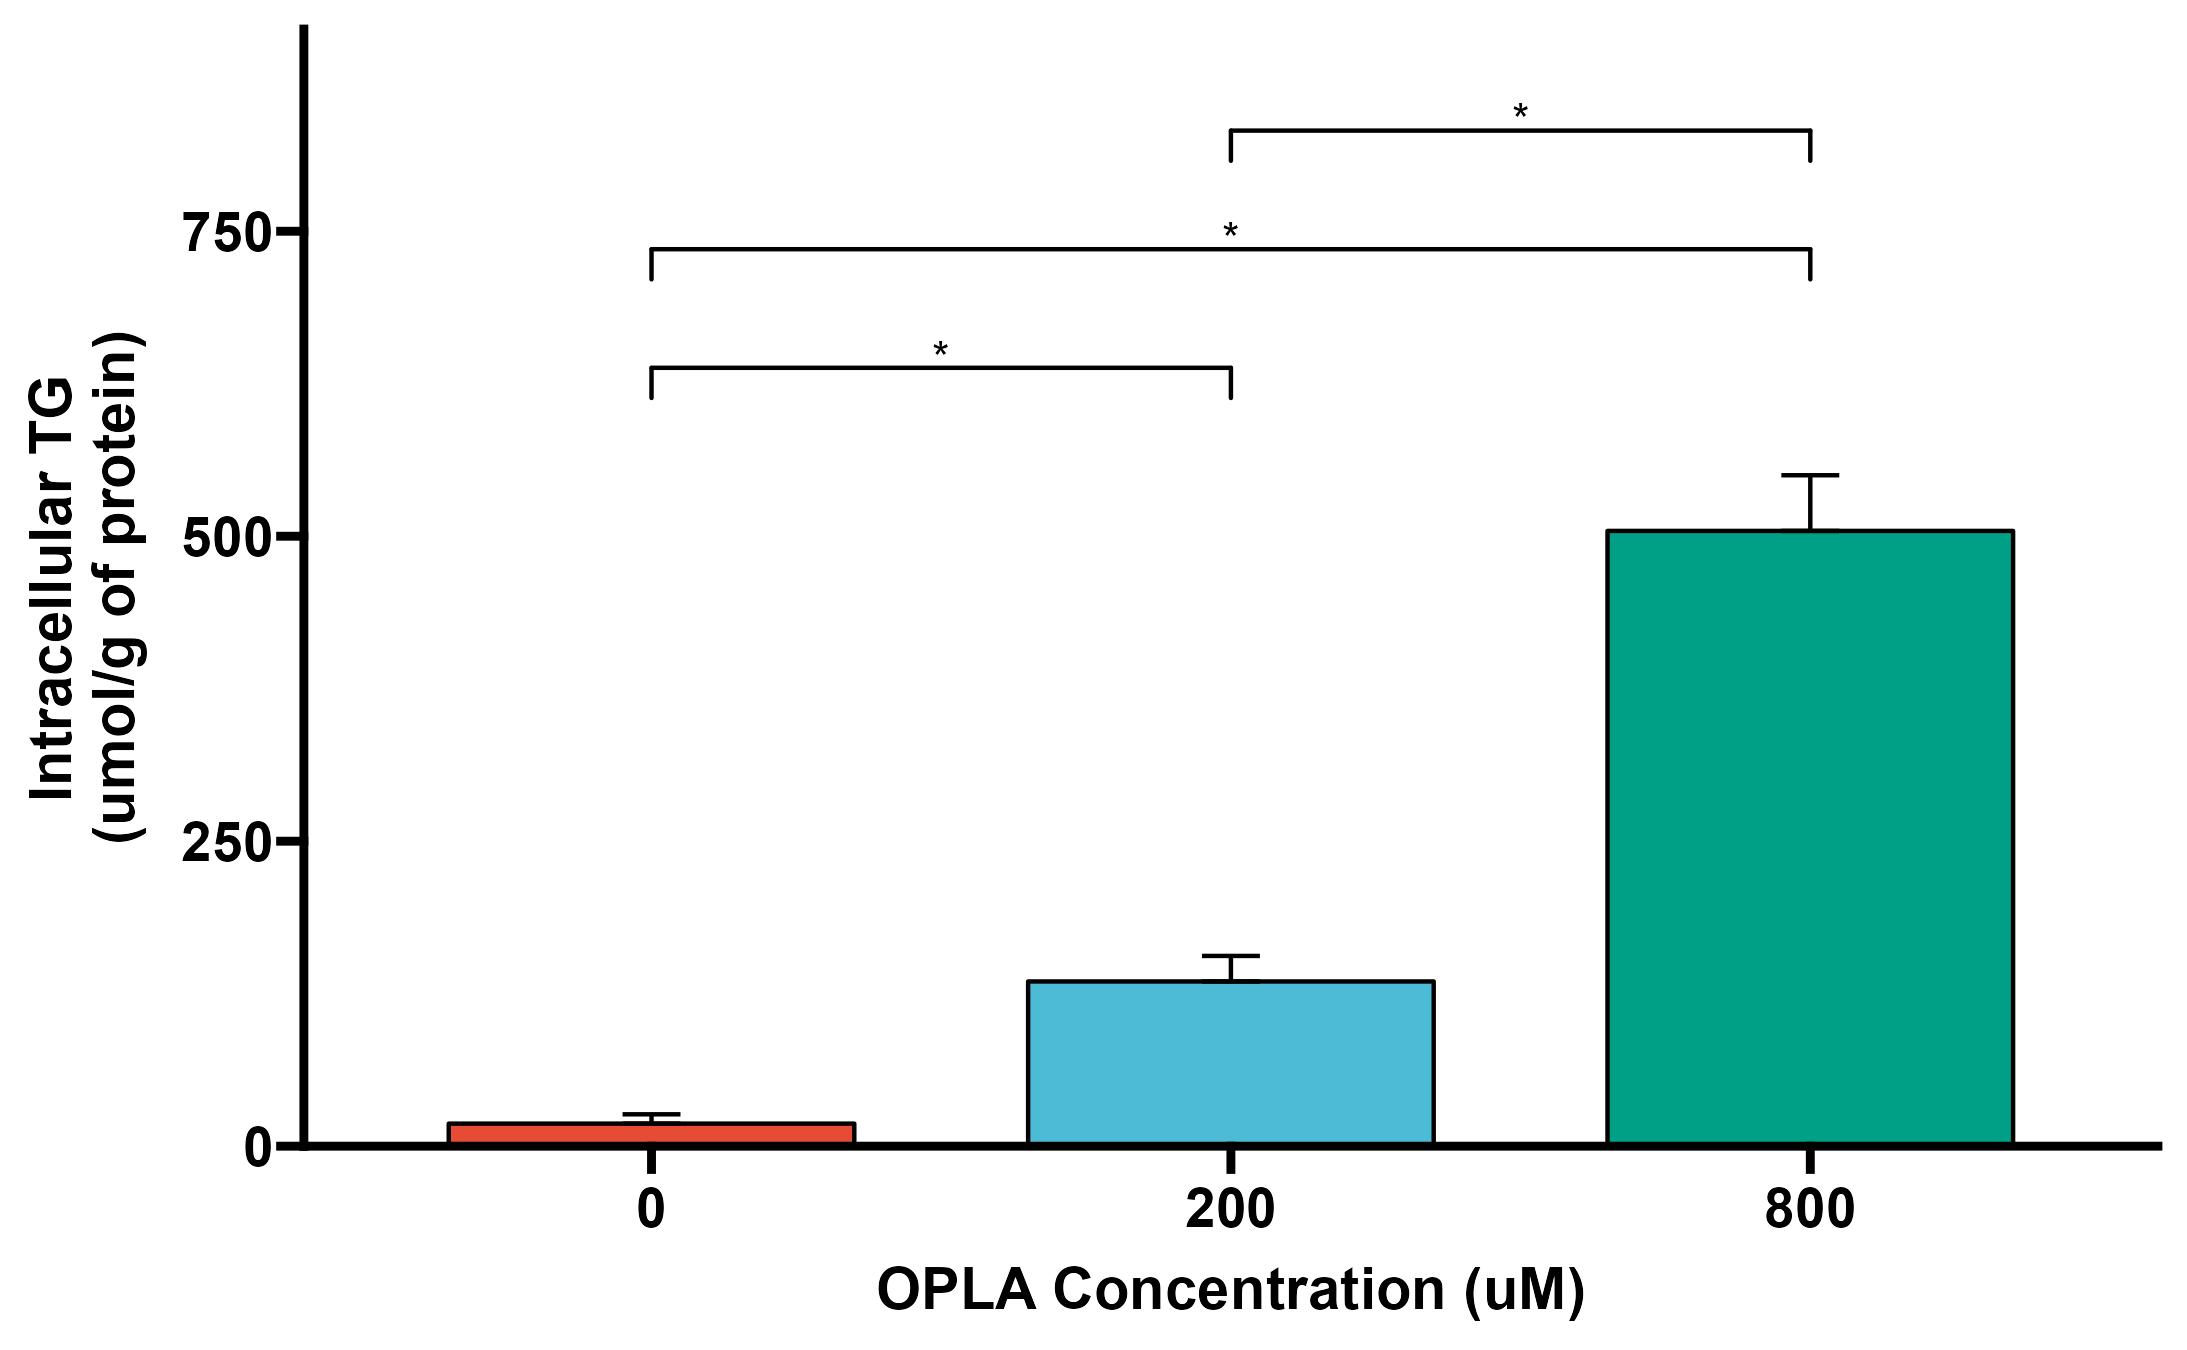
\includegraphics[width=\textwidth]{figures/ch3-Model Development/LFHF TG.png}
     \end{subfigure}  
     \hfill
     \begin{subfigure}[b]{0.49\textwidth}
         \textbf{B}
         \centering
         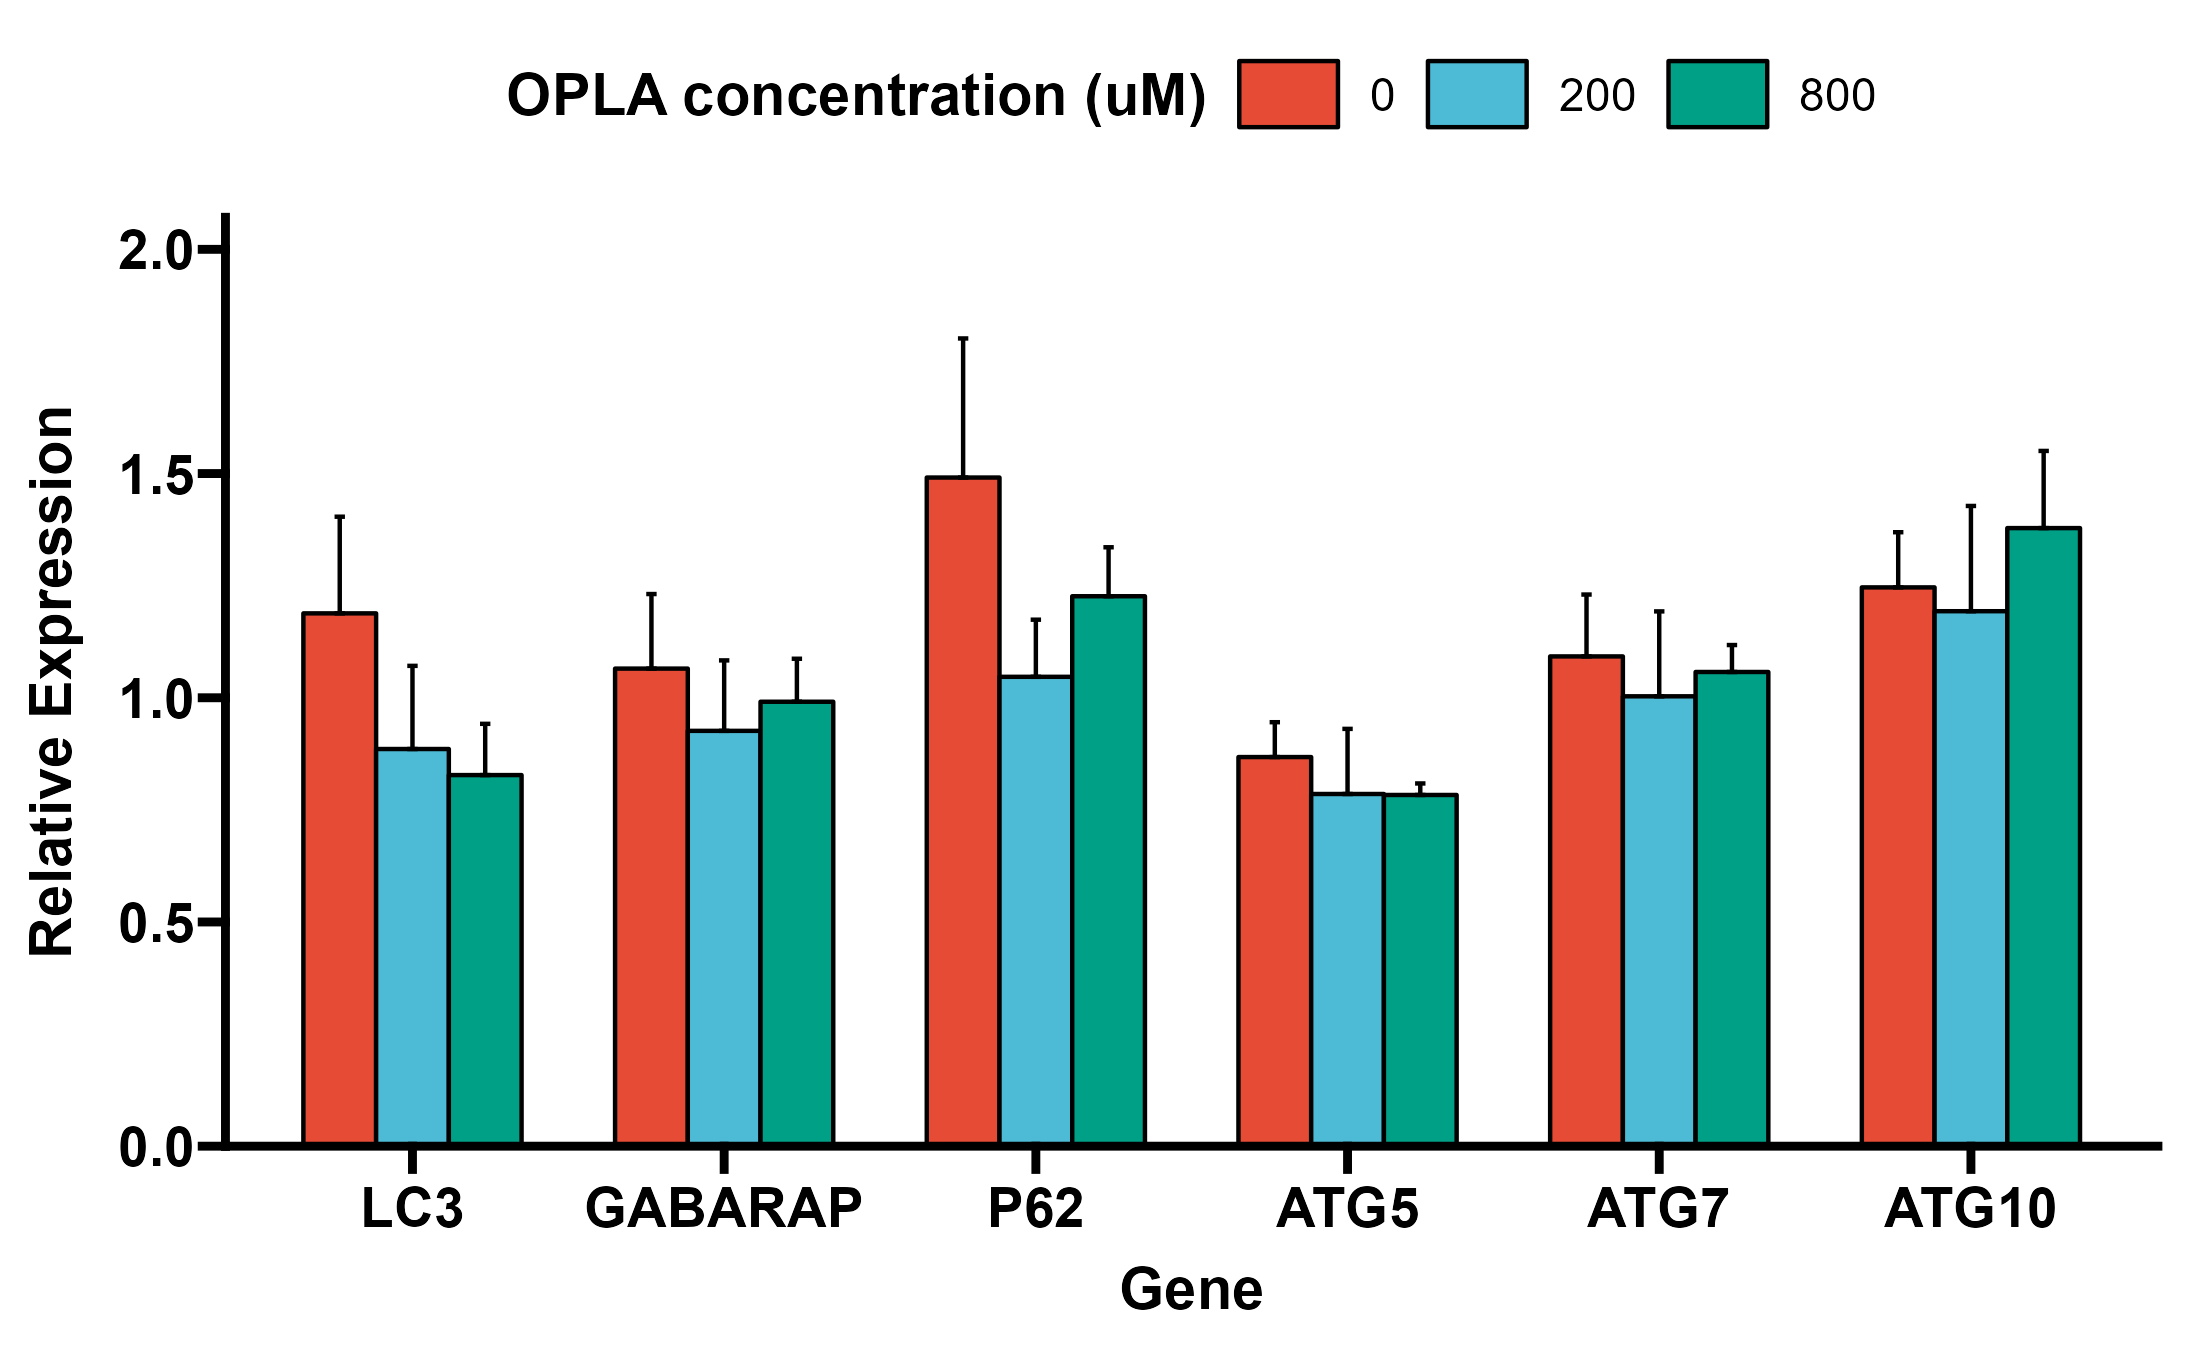
\includegraphics[width=\textwidth]{figures/ch3-Model Development/LFHF ATG genes.png}
     \end{subfigure}
     \hfill
        \caption{Effect of media FA concentration on intracellular triglyceride content (a) and autophagic gene expression (b). Representative of three biological repeats (n=3) carried out in technical triplicate. * = p-value < 0.05. Abbreviations: TG, Triglyceride.}
        \label{fig:ch3-Model Development LFHF}
\end{figure}